\paragraph{Historical and designed artefacts.} In order to understand how our brain works or could work, we must possess conceptual clarity --- we must conceive of it, not as a product of one-time engineering, but as a historical artefact. Unlike ``perfect'' systems, like Peano arithmetic and the $\lambda$ calculus, those which grew historically does not make sense if one only looks at their current snapshot. One will find nonsensical solutions, and kludge piled on top of kludge in a futile attempt to correct some early erroneous design decision. The system as a whole will operate according to incomprehensible schemata and be ensouled with a mad logic of which no sane engineer would ever conceive. Of all such systems, the human brain might well be the most complex one; the task of understanding it correspondingly harrowing. More than one AI researcher despaired at it and said that the brain simply has no architecture at all \cite[p. \todo{page}]{norvig}:

\begin{quotation}
	\todo{insert quote here}
\end{quotation}

It the classical sense, it probably does not, but one can relax the notion of ``architecture'' to include structures that result from incremental change and the creative combination of pre-existing parts. While the results of such processes are often extremely unintuitive and often even incomprehensible to us, we at least have a way of understanding them by re-tracing their evolution. Doing so is laborious. Doing so is laborious and requires a huge amount of data (which we currently do not have), but this approach of regarding brain function as through-and-through Darwinian might results that have, so far, eluded the other schools of thought in the field.

What, one might ask, is the consequence of such a view? The first is that each new feature in the developmental history had to have been useful on its own. The second is that it allows the distinction between what I will herein call \textsc{efficient} systems and \textsc{clean} systems. Since, at each stage of its evolution, the organism that carried the brain had to be viable, the end product is by definition guaranteed to be ``efficient''. Because of that same fact, however, it is all but guaranteed not to be ``clean'': for one, it was not possible to snap whole new components into the system; it would have also been impossible to combine old components in the elaborate and precise ways in which a human engineer might use parts. Worse, old components were almost certainly not discarded when new and better ones came into being. A good exposition of this process in humans can be found in Paul MacLean's seminal work {\em The Triune Brain in Evolution} \cite{maclean1990}.


\todo{sodium channels as precursors to neurons (brains?) w.r.t. F in fig. 2}
\begin{figure}[!h]
	\centering
	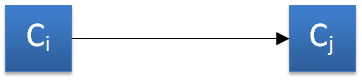
\includegraphics{figs/noNervousSystem.png}
	\caption{Relationship between the components of an organism without a nervous system.}
	\label{fig:noNervousSystem}
\end{figure}
%\vspace{-0.18cm}
\subsection{Origin of nervous systems} The evolution of nervous systems in organisms dates back to the development of primitive electrical signalling in eukaryotes, using calcium action potentials\footnote{See any textbook on evolutionary biology.} and sodium channels \cite{Liebeskind31052011}:

\begin{quotation}
	Voltage-dependent sodium channels are believed to have evolved from calcium channels at the origin of the nervous system.
\end{quotation}

These sodium channels predated modern-day neurons, but served the same fundamental purpose of acting as control systems. We can readily conceive the benefits of imparting a control system onto an organism with the following thought experiment: let us imagine a microscopic organism without any sort of nervous system --- all of its behaviour is hard-coded and mechanical. It can take in nutrients through its cell walls or through an opening; parts of it can contract or expand in response to stimuli like light or pressure; homeostatic conditions can influence its chemistry. Figure~\ref{fig:noNervousSystem} shows this schema: if we enumerate the constituent parts or {\em components} of an organism as $\{C_1,\dots,C_n\}$, the organism's behavior is caused by signals being sent between $C_i$ and $C_j$ (the case $i=j$ is possible). Such an organism suffers from three disadvantages: (a) reactions are localized, as two of its components might be too far apart to communicate in a timely manner or at all; (b) its repertoire of behaviours is necessarily simple and (c) it is not very adaptable.

Precursors to nervous systems ameliorated (a) first via action potentials, which were intracellular electrical signals \cite{Liebeskind31052011} (emphasis mine):
\begin{quotation}
Another key animal innovation was the nervous system, which is present in all but a few animals (i.e., sponges and placozoans). {\em Rapid, specific, long-distance communication among excitable cells} is achieved in bilaterian animals and a few jellyfish (cnidarians) through the use of action potentials (APs) in neurons generated by voltage-dependent sodium (Na$_\mathrm{v}$) channels. Voltage dependent calcium (Ca$_\mathrm{v}$) channels evolved in single-celled eukaryotes and were used for intracellular signaling. {\em It has been hypothesized that Na$_v$ channels were derived from Ca$_v$ channels at the origin of the nervous system} \textsf{[the results in the paper support the hypothesis]} (3), thereby conferring the ability to conduct action potentials without interfering with intracellular calcium. This view was reinforced by the apparent lack of sodium currents in sponges (4).
\end{quotation}

The introduction of dedicated, long-distance\todo{add source}\footnote{The term ``long-distance'' may very well mean ``long-distance within a single cell''. Franti\v{s}ek and Mancuso argue in \cite{frantisek} that neural analogues already existed in prokaryotes and unicellular eukaryotes.} signalling cells between parts of an organism created the possibility of not only transmitting, but also modifying information. The moment an organism's parts do not communicate directly biochemically/mechanically, but over transmissions lines, evolutionary processes acting upon these lines are able to mutate them so that they change the signals. The first changes might consist of amplifying, diminishing, or distributing signals. Over time, the nerves may come to act as transducers on the stream of signals; in some rudimentary sense, they may begin to compute functions. Schematically, we see this in Figure~\ref{fig:nervousSystem}, where a function $F$ is interposed between two components. Not all components of an organism are created equal, of course. The first and most important use of nerve cells was the communication between sensory organs and the movement apparatus of the organism, and the bulk of nerve cells were located close to the sensory organs, where they processed information. A mere handful of neurons are not able to compute much, but they must have conferred considerable advantage to their owners.

\begin{figure}
	\centering
	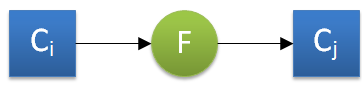
\includegraphics{figs/nervousSystem.png}
	\caption{Relationship between the components of an organism possessing a nervous system. $F$ can be understood as a simple signal transformer or a central coordinating mechanism.}
	\label{fig:nervousSystem}
\end{figure}

The history of these developments is not entirely clear, but action potentials are present in all animals (with the exception of sponges) and in plants \cite{Leys01051999, PCE:PCE1614}. 
A step up from mere stream transducers are the nerve nets that permeate the entire bodies of cnedaria (jellyfish) and the nerve cords that run along the bodies of bilateria (animals with left and right sides). In Figures~\ref{fig:animalia} and \ref{fig:animalia2} we see the phylogeny of the animalia kingdom.

\begin{figure}
	\centering
	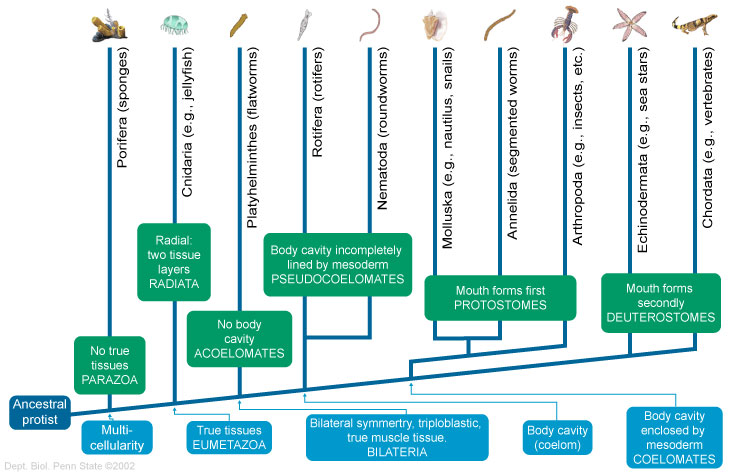
\includegraphics[width=\textwidth]{Figs/animalia.jpg}
	\caption{Phyolgeny of the animalia. Note the cnidaria and bilateria; both of these have types of nervous systems. From \cite{animalia}.}
	\label{fig:animalia}
\end{figure}

\begin{figure}
	\centering
	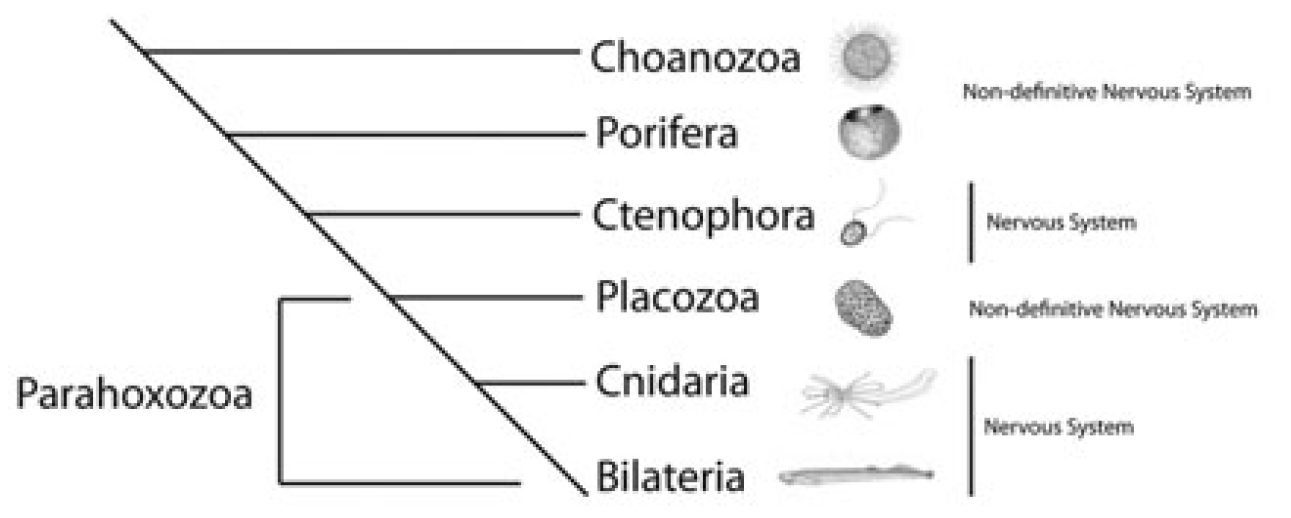
\includegraphics[width=\textwidth]{Figs/animalia2.png}
	\caption{Phyolgeny of the animalia. Even Ctenophores, macroscopic marine invertebrates which predate both jellyfish and bilateria, have nervous systems in the form of distributed nerve nets. From \cite{animalia2}.}
	\label{fig:animalia2}
\end{figure}

\todo{put in the graphics of nerve nets and nerve cords}

\todo{go to higher animal and human intelligence}

\paragraph{Implications} The point in all this is not to give an exhaustive overview of evolutionary neurobiology; it is to show that nervous systems are ancient, gradually developed things. They have been shaped by the vicissitudes of hundreds of millions of years, and they could have developed in other ways. They were not planned, as a human would understand to word. If we are to gain headway in piecing together the ``big picture'', we must take these facts to heart, and choose our modelling methods accordingly.

In the abstract of this work, I described the biological and the idealistic approaches as being polar opposites, and this is true as far engineering is concerned, but in terms of their assumptions, false. They are both idealistic. Neural networks, insofar as their users want to re-create human behaviour, implicitly presuppose an intelligence in neurons that is not there. The comparatively small network is taught to compute some desired function, the hope being that it might thereby come to perform some complex, real-world function like common-sense reasoning. In principle, this strategy could work, but in practice, it is unrealistic --- the environment in which real organisms had to succeed was the planet's ecosphere; billions upon billions of nervous systems of all complexities were run over millions of years; nervous systems died off and were re-created from scratch by genes. It is therefore entirely unreasonable to assume that neural network, trained against an objective function over a period of hours or days could re-create the function a biological organism, unless one were to suppose that there is some inherent quality in neurons that strives for such; that groups of cells somehow {\em wish} to organize themselves into specific configurations in which they are able to perform activities we would call ``cognition''. 

All this being said, we should not confuse criticism of the suitability of a method for a specific purpose with criticism of its suitability for any purpose. Neural networks have proven useful in understanding mental activity at small scales; both they and the symbolic/logic-based approaches have had a myriad of industrial applications. From this, however, it does not follow that we can build genuinely intelligent agents with them. Our only means of doing that (the only means that remain) is to laboriously unravel the developmental history of animal brains, step by step, making sense of each development in context. Where empirical data are not available, we at least have to hypothesize how things could plausibly have happened. To day, structural and genetic analyses have been done (via genetic sequencing and MRI), but they do not deliver sufficiently detailed data. Such methods are rather akin to measuring voltages and task time in a PC --- they do tell us something, but an observer would never infer the existence of e.g. compilers, call stacks, or type systems from such observations. For an understanding of the brain so specific that we can re-implement it in a computer, we will need currently non-existent and not-conceived-of technology. Until that day --- and this will be the main thrust of this thesis --- guesswork will have to suffice.

\subsection{Ways of adaptation}

The neuron bundles would have been quite malleable in the face of selection pressure: when the environment required it, they could, after several generations, start to compute different or more elaborate functions. For instance, an organism which had had developed in an environment where food was abundant in bright places and which had now found itself in darkness would have benefited from a variety of plausible changes, such as
\begin{itemize}
	\item an inversion of its light-seeking behaviour,
	\item switching off its metabolism in light places to conserve energy,
	\item accelerating its metabolism in dark places to make better use of the food there.
\end{itemize}

Of course, other changes would have also been possible, such as the metabolization of different food sources,\footnote{A current-day example is given by nylon-eating bacteria, which have developed in the last century and which now have an abundant food source and no competition.} but we can see how the aforementioned three could have been effected through changes in a simple nervous system alone. Let us recall the beginning of this section and contrast such a malleable computational mesh with most products of human engineering: one cannot simply take out a piston in a car or replace a cogwheel in a mechanical clock with a differently sized one. Machines are designed to fit together perfectly and their complexity tends to be irreducible. Even programs, which are more open to mutation and which are often evolved in evolutionary algorithms, are easily broken by small changes.

\paragraph{Adaptation of nervous systems}  When discussing how an organism's nervous system can evolve and, in particular, {\em evolve to perform new tasks} and not just variations on old ones, explanations are again constrained by two criteria: (a) the change has to be small, or at least have a small cause\footnote{The effect does not have to be small --- changes in single genes can switch entire components on or off. The MYH16 gene, which is present in non-human primates but has been switched off in humans, is an example. In us, its disabling lead to a drastic reduction in the size of jaw muscles and a corresponding increase in brain size~\cite{carroll2005}.} and (b) each change must be beneficial in the short term.\footnote{Caveats apply: if the selection pressure on a group of organisms isn't too strong, changes which may be sub-optimal but perhaps beneficial at some later point may spread, and non-selective processes like genetic drift can also play a role.}

To illustrate this, we can look at a simple neural network in Figure~\ref{fig:neuralNetwork}, with a marked node $N_x$. Figure~\ref{fig:unlikelyEvolution} shows an unlikely change scenario in which some new component/function is cleanly grafted onto the system. Figure~\ref{fig:likelyEvolution} then shows a much more likely scenario: a mutation causes $N_x$ to be split and the new nodes take over some of its connections. In time, new functions can thus grow into the system, but never in the manner in which, say, an engineer would implement a new feature.

\begin{figure}
	\centering
	\begin{subfigure}[t]{0.45\textwidth}
		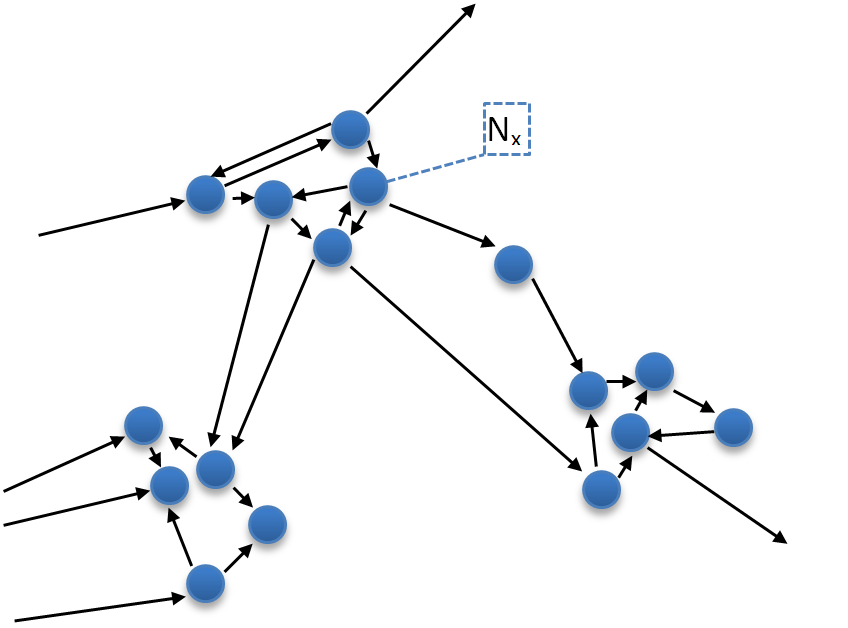
\includegraphics[width=\textwidth]{figs/neuralNetwork.png}
		\caption{A simple neural network.}
		\label{fig:neuralNetwork}
	\end{subfigure}
	\begin{subfigure}[t]{0.45\textwidth}
		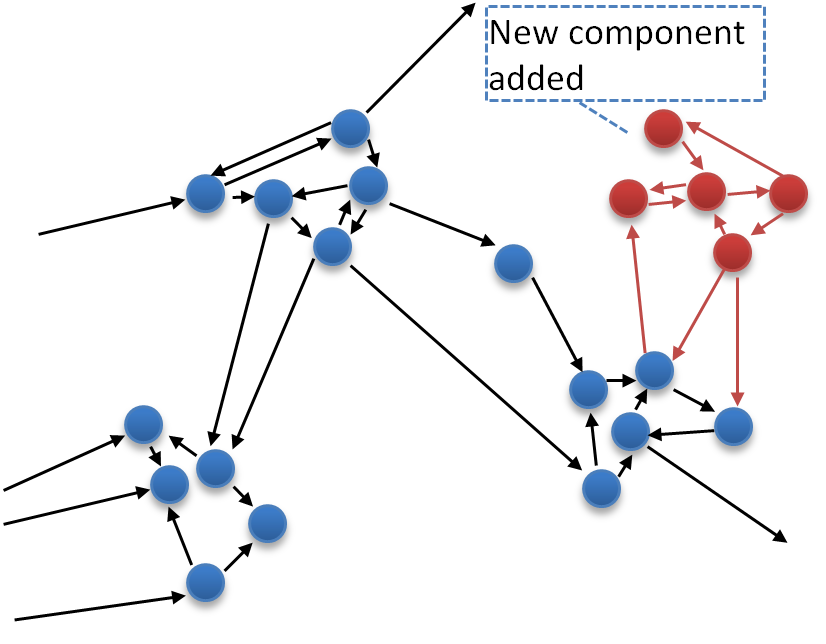
\includegraphics[width=\textwidth]{figs/unlikelyEvolution.png}
		\caption{An unlikely change scenario in which new, discernible components are grafted on from whole cloth.}
		\label{fig:unlikelyEvolution}
	\end{subfigure}
	\begin{subfigure}[t]{0.45\textwidth}
		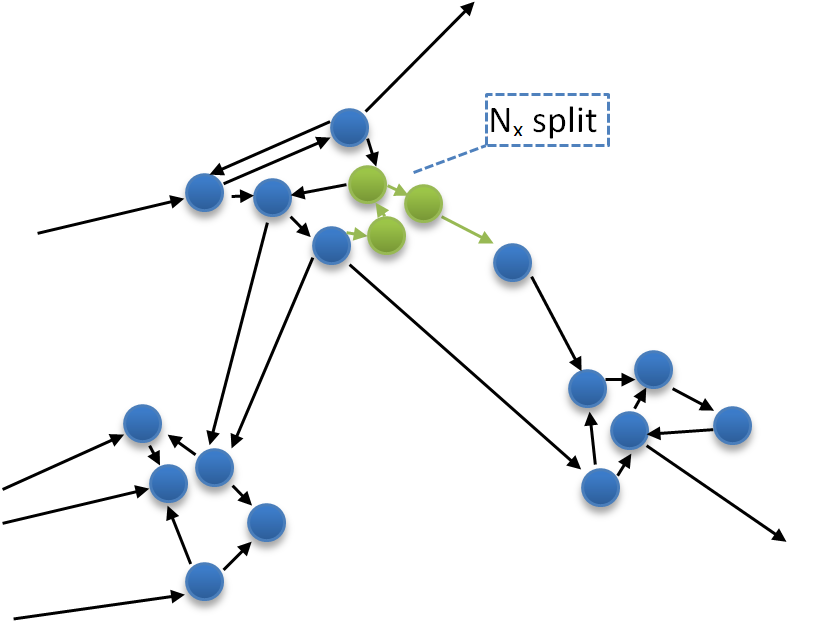
\includegraphics[width=\textwidth]{figs/likelyEvolution.png}
		\caption{A more likely change scenario in which one part is split into three but where the overall shape of the network is not appreciably altered.}
		\label{fig:likelyEvolution}
	\end{subfigure}
\end{figure}

\paragraph{The brain as a collection of functions}

The processes hitherto described are quite uncontroversial and can be found reiterated in any textbook on the evolution of nervous systems. The functional structure and the model of computation used in the brain, however, are not well understood. FMRI and similar brain imagining techniques, while invaluable, give only rough impressions about the neural correlates of certain forms of cognition and do not give fine-grained insight into its structure. As such, the model I shall describe in the following paragraphs is a conjecture. The implication of such an evolutionary viewpoint, I conjecture in this document, is that brain functions don't ``just appear'', but are rather the result of small changes and the recombination of pre-existing parts. This, in turn, informs the plausibility of various possible brain architectures. In becomes unlikely that the brain should be a collection of neatly delineated functions, or that it should have certain coordinating units or universal message formats for communication between components. The reason for this is that administrative mechanism confer little evolutionary benefit on their owen, and do not confer it gradually: the imposition of a central coordinating mechanism on a pre-existing mesh of neurons would necessitate the complete reorganisation of such, and the abandonment of the previous communication channels on favor centralized coordination. The same objections can be raised against a universal or even a local message format. Moreover, such mechanisms require substantial changes in the organism with no obvious or immediate advantage.

Such objections do not contradict the existence of macroscopic structures in the brain, dedicated to certain tasks. The development and adaptation of such remains entirely plausible. They do, however, give insight into the pattern of processing inside such structures, which is often simply regarded as atomic or replicated in computers as if it were a conventional engineering product.

Instead of a rigidly ordered brain with central organisation and large, discrete, and highly complex features like ``sight'' or ``reason'' which function like pluggable black boxes, I propose a decentralized white-box architecture composed of simple parts: first, every component, while perhaps sophisticated, is conceptually simple. Second, communication between different components is not performed in the function-call pattern of computer programs, but rather by one component listening in on the activity of another. Since there is, inherently, no mechanism of function abstraction in neural systems, it stands to reason that the most likely way for new functions to develop is for additional neurons to modulate the activity of others. In such a scheme, a visual perception component does not have to know which other components will consume its output (or rather, listen on its activity); changes which affect agent activity in useful ways based on the visual data can occur gradually and, over time, become large enough to count as components in their own right.

\paragraph{Practical abstraction}

While such a white-box model is conceptually useful, a mesh of gradually grown patterns does not lend itself to implementation in a program. Therefore, I will present a simplified model which, while attempting to remain true to the conceptual view, will, pragmatically, contain discrete functions and components. The white-box nature of brain activity will be emulated by a message-passing scheme in which messages model the internal activity of components. Instead of each component blindly acting in some fashion on the activity of another, components will have explicit parsers and interpreters and later, these will be further simplified into localized message formats and tagging, for the sake of easy implementation.